%%=============================================================================
%% Methodologie
%%=============================================================================

\chapter{\IfLanguageName{dutch}{Methodologie}{Methodology}}%
\label{ch:methodologie}

%% TODO: In dit hoofstuk geef je een korte toelichting over hoe je te werk bent
%% gegaan. Verdeel je onderzoek in grote fasen, en licht in elke fase toe wat
%% de doelstelling was, welke deliverables daar uit gekomen zijn, en welke
%% onderzoeksmethoden je daarbij toegepast hebt. Verantwoord waarom je
%% op deze manier te werk gegaan bent.
%% 
%% Voorbeelden van zulke fasen zijn: literatuurstudie, opstellen van een
%% requirements-analyse, opstellen long-list (bij vergelijkende studie),
%% selectie van geschikte tools (bij vergelijkende studie, "short-list"),
%% opzetten testopstelling/PoC, uitvoeren testen en verzamelen
%% van resultaten, analyse van resultaten, ...
%%
%% !!!!! LET OP !!!!!
%%
%% Het is uitdrukkelijk NIET de bedoeling dat je het grootste deel van de corpus
%% van je bachelorproef in dit hoofstuk verwerkt! Dit hoofdstuk is eerder een
%% kort overzicht van je plan van aanpak.
%%
%% Maak voor elke fase (behalve het literatuuronderzoek) een NIEUW HOOFDSTUK aan
%% en geef het een gepaste titel.

Dit onderzoek hanteert een empirisch-technische aanpak op basis van experimentele validatie met kwantitatieve metrieken. Deze keuze past bij de onderzoeksvraag: om uitspraken te doen over detectienauwkeurigheid en tijdsbesparing zijn meetbare resultaten nodig die reproduceerbaar zijn. Het onderzoek verloopt in vier opeenvolgende fasen die op elkaar voortbouwen: een literatuurstudie legt het theoretische fundament, een requirementsanalyse vertaalt compliance-eisen naar concrete criteria, een prototypingfase realiseert het framework, en een validatiefase meet de effectiviteit ervan. Figuur~\ref{fig:methodologie_flow} geeft een schematisch overzicht van deze doorlopen fasen en de iteratieve feedbacklus tussen validatie en ontwerp.

% --- TIKZ FLOWCHART ---
\begin{figure*}[htbp]
    \centering
    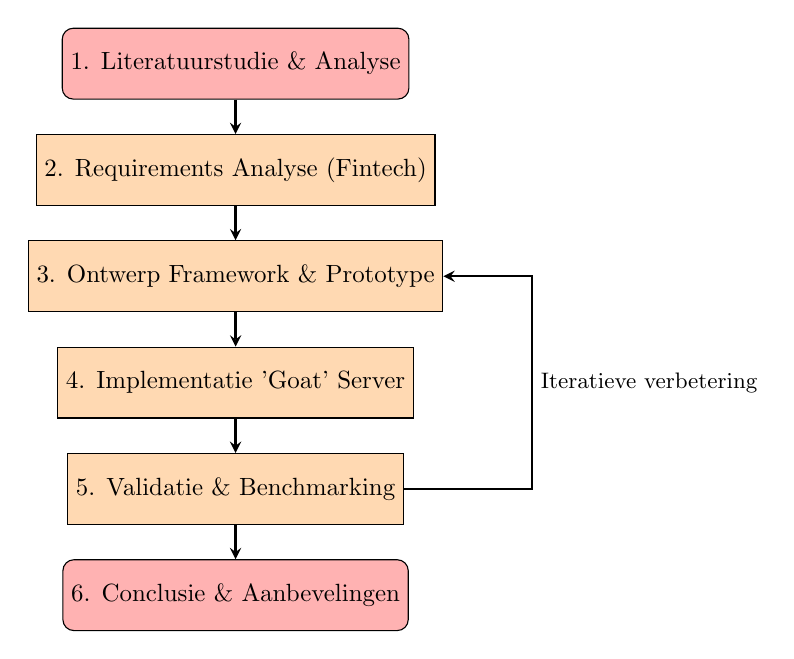
\begin{tikzpicture}[node distance=1.5cm, scale=0.9, transform shape]
        % Stijlen definiëren
        \tikzstyle{startstop} = [rectangle, rounded corners, minimum width=3cm, minimum height=1cm, text centered, draw=black, fill=red!30]
        \tikzstyle{process} = [rectangle, minimum width=3cm, minimum height=1cm, text centered, draw=black, fill=orange!30]
        \tikzstyle{io} = [trapezium, trapezium left angle=70, trapezium right angle=110, minimum width=3cm, minimum height=1cm, text centered, draw=black, fill=blue!30]
        \tikzstyle{arrow} = [thick,->,>=stealth]

        % Knopen plaatsen
        \node (lit) [startstop] {1. Literatuurstudie \& Analyse};
        \node (req) [process, below of=lit] {2. Requirements Analyse (Fintech)};
        \node (design) [process, below of=req] {3. Ontwerp Framework \& Prototype};
        \node (poc) [process, below of=design] {4. Implementatie 'Goat' Server};
        \node (test) [process, below of=poc] {5. Validatie \& Benchmarking};
        \node (concl) [startstop, below of=test] {6. Conclusie \& Aanbevelingen};

        % Pijlen trekken
        \draw [arrow] (lit) -- (req);
        \draw [arrow] (req) -- (design);
        \draw [arrow] (design) -- (poc);
        \draw [arrow] (poc) -- (test);
        \draw [arrow] (test) -- (concl);

        % Feedback loop
        \draw [arrow] (test.east) -- ++(1.8,0) |- (design.east) node[pos=0.25, right, font=\small] {Iteratieve verbetering};

    \end{tikzpicture}
    \caption{Schematische weergave van de onderzoeksstappen.}
    \label{fig:methodologie_flow}
\end{figure*}

\section{Fase 1: Literatuurstudie en classificatie van dreigingen}

De eerste fase bestaat uit een literatuurstudie via academische databanken (Google Scholar, IEEE Xplore, arXiv) en officiële technische documentatie. De architectuur en datastromen van MCP worden doorgrond, en bestaande taxonomieën van AI-kwetsbaarheden --- zoals de OWASP Top 10 voor LLM's --- worden geanalyseerd op relevantie voor de MCP-context. Het concrete doel is een kwetsbaarheidstaxonomie opstellen voor prompt injection, tool poisoning en privilege escalation in financiële toepassingen. De resultaten vormen het hoofdstuk Stand van zaken. Geschatte doorlooptijd: vier weken.

\section{Fase 2: Requirementsanalyse voor Fintech-toepassingen}

De requirementsanalyse steunt op documentanalyse van compliance-kaders (PCI-DSS, GDPR) en API-security best practices, niet op interviews of enquêtes. Die keuze is bewust: harde compliance-eisen leveren objectievere criteria op dan subjectieve meningen. De functionele en niet-functionele vereisten --- waaronder logging, auditability en toegangscontrole --- worden ingedeeld via de MoSCoW-methode en gedocumenteerd in het hoofdstuk Requirementsanalyse. Geschatte doorlooptijd: twee weken.

\section{Fase 3: Ontwerp en implementatie van het assessment framework}

In de derde fase wordt het framework gebouwd als een modulaire Python-applicatie. Python is gekozen vanwege de native ondersteuning voor JSON-RPC en asynchrone communicatie, beide vereist voor MCP. Het framework bestaat uit drie kerncomponenten:

\begin{enumerate}
    \item \textbf{Discovery Module:} Analyseert de \texttt{list\_tools} en \texttt{list\_prompts} endpoints.
    \item \textbf{Static Analysis Engine:} Scant tool-beschrijvingen op onveilige patronen.
    \item \textbf{Dynamic Probing Engine:} Voert actieve fuzzing uit met gemanipuleerde payloads.
\end{enumerate}

De implementatie maakt gebruik van Python~3.12, Docker, Pydantic en de officiële \texttt{mcp}-library. Het resultaat is een werkende Proof of Concept gepubliceerd als open-source code op GitHub. Geschatte doorlooptijd: zes weken.

\section{Fase 4: Validatie via een 'Vulnerable MCP Server'}

Omdat er weinig publieke testdata beschikbaar is, wordt een eigen testomgeving ontwikkeld: de \emph{Fintech MCP Goat}, een opzettelijk kwetsbare MCP-server die financiële scenario's nabootst (saldo opvragen, overschrijving starten). Deze server dient als gecontroleerde \emph{ground truth}. Parallel wordt een gestructureerde handmatige beoordelingsprocedure vastgelegd als checklist, zodat de vergelijking reproduceerbaar is. Per testscenario worden vier grootheden gemeten:

\begin{itemize}
    \item \textbf{Detectieratio (Recall):} $\frac{\text{Aantal gevonden kwetsbaarheden}}{\text{Totaal aantal aanwezige kwetsbaarheden}}$, gemeten voor zowel de handmatige review als het framework
    \item \textbf{False Positive Rate:} Aantal onterechte alarmen voor beide methoden
    \item \textbf{Performance:} Benodigde tijd voor volledige assessment (handmatig in uren, geautomatiseerd in minuten)
    \item \textbf{Kwalitatieve analyse:} Identificatie waar menselijke expertise beter presteert (contextuele interpretatie) versus waar de tool superieur is (herhaalbaarheid, volledigheid)
\end{itemize}

De testomgeving draait via Docker~Compose; Burp~Suite wordt ingezet voor manuele verificatie. Het resultaat is een validatierapport met kwantitatieve meetresultaten. Geschatte doorlooptijd: drie weken.

\section{Overzichtstabel Planning}

Tabel~\ref{tab:planning} geeft een samenvattend overzicht van de fasering en deliverables.

\begin{table*}[htbp]
    \centering
    \caption{Planning en deliverables per onderzoeksfase.}
    \label{tab:planning}
    \begin{tabular}{@{}llp{6cm}@{}}
        \toprule
        \textbf{Fase}       & \textbf{Duur} & \textbf{Deliverable}               \\ \midrule
        1. Literatuurstudie & 4 weken       & Dreigingsmodel \& State-of-the-art \\
        2. Requirements     & 2 weken       & Requirementslijst (MoSCoW)         \\
        3. Implementatie    & 6 weken       & Python Framework (GitHub repo)     \\
        4. Validatie        & 3 weken       & Validatierapport \& Testresultaten \\
        5. Conclusie        & 2 weken       & Finaliseren Bachelorproef tekst    \\ \bottomrule
    \end{tabular}
\end{table*}

